\documentclass[11pt,twoside,a4paper]{article}
% http://www-h.eng.cam.ac.uk/help/tpl/textprocessing/latex_maths+pix/node6.html symboles de math
% http://fr.wikibooks.org/wiki/Programmation_LaTeX Programmation latex (wikibook)
%=========================== En-Tete =================================
%--- Insertion de paquetages (optionnel) ---
\usepackage[french]{babel}   % pour dire que le texte est en fran{\'e}ais
\usepackage{a4}	             % pour la taille   
\usepackage[T1]{fontenc}     % pour les font postscript
\usepackage{epsfig}          % pour gerer les images
%\usepackage{psfig}
\usepackage{amsmath, amsthm} % tres bon mode mathematique
\usepackage{amsfonts,amssymb}% permet la definition des ensembles
\usepackage{float}           % pour le placement des figure
\usepackage{verbatim}

\usepackage{multicol} % multicolonnes

\usepackage{longtable} % pour les tableaux de plusieurs pages

\usepackage[table]{xcolor} % couleur de fond des cellules de tableaux

\usepackage{lastpage}

\usepackage{multirow}

\usepackage{multicol} % pour {\'e}crire dans certaines zones en colonnes : \begin{multicols}{nb colonnes}...\end{multicols} 

% \usepackage[top=1.5cm, bottom=1.5cm, left=1.5cm, right=1.5cm]{geometry}
% gauche, haut, droite, bas, entete, ente2txt, pied, txt2pied
\usepackage{vmargin}
\setmarginsrb{0.20cm}{0.20cm}{0.20cm}{0.20cm}{15pt}{3pt}{15pt}{3pt}

\usepackage{lscape} % changement orientation page
%\usepackage{frbib} % enlever pour obtenir references en anglais
% --- style de page (pour les en-tete) ---
\pagestyle{plain}

% % % en-tete et pieds de page configurables : fancyhdr.sty

% http://www.trustonme.net/didactels/250.html

% http://ww3.ac-poitiers.fr/math/tex/pratique/entete/entete.htm
% http://www.ctan.org/tex-archive/macros/latex/contrib/fancyhdr/fancyhdr.pdf
% \usepackage{fancyhdr}
% \pagestyle{fancy}
% % \newcommand{\chaptermark}[1]{\markboth{#1}{}}
% % \newcommand{\sectionmark}[1]{\markright{\thesection\ #1}}
% \fancyhf{}
% \fancyhead[LE,RO]{\bfseries\thepage}
% \fancyhead[LO]{\bfseries\rightmark}
% \fancyhead[RE]{\bfseries\leftmark}
% \fancyfoot[LE]{\thepage /\pageref{LastPage} \hfill
	% TITLE
% \hfill 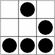
\includegraphics[width=0.5cm]{img/logo_glider.png} }
% \fancyfoot[RO]{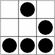
\includegraphics[width=0.5cm]{img/logo_glider.png} \hfill
	% TITLE
% \hfill \thepage /\pageref{LastPage}}
% \renewcommand{\headrulewidth}{0.5pt}
% \renewcommand{\footrulewidth}{0.5pt}
% \addtolength{\headheight}{0.5pt}
% \fancypagestyle{plain}{
	% \fancyhead{}
	% \renewcommand{\headrulewidth}{0pt}
% }

\def\smallbox{%
	\setlength{\unitlength}{0.5cm}
	\fbox{
		\begin{picture}(1, 1)(0,0)
		\end{picture}
	}
}%

%%%%%%%%%%% SOME VALUES IN ENGLISH %%%%%%%%%%%%%%%%%%%%%
\def\ENdefFichePerso{Character Sheet}
\def\ENdefNom{\textbf{Name} \dotfill }
\def\ENdefDateCreation{\textbf{Date of creation} \_\_/\_\_/\_\_\_\_ }
\def\ENdefTaille{\textbf{Height} \dotfill }
\def\ENdefPoid{\textbf{Weight} \dotfill }
\def\ENdefTotalPoints{\textbf{Point Total} \dotfill }
\def\ENdefRestePoints{\textbf{Unspent Points} \dotfill }
\def\ENdefJoueur{\textbf{Player} \dotfill }
\def\ENdefCampagne{\textbf{Campaign} \dotfill }
\def\ENdefModificateurTaille{\textbf{Size Modifier} \dotfill }
\def\ENdefAge{\textbf{Age} \_\_\_}
\def\ENdefApparenceMain{\textbf{Appearance} \dotfill }
\def\ENdefCourant{{\footnotesize \textsc{current}}}
\def\ENdefFO{ST}	% ST
\def\ENdefDX{DX}	% DX
\def\ENdefQI{IQ}	% IQ
\def\ENdefSA{HT}	% HT
\def\ENdefPV{HP}	% HP
\def\ENdefVOL{WILL}	% WILL
\def\ENdefPER{PER}	% PER
\def\ENdefPS{FP}	% FP
\def\ENdefBasePortage{Basic Lift \dotfill }
\def\ENdefBaseVitesse{Basic Speed \dotfill  [~~]}
\def\ENdefBaseMove{Basic Move \dotfill  [~~]}
\def\ENdefDommage{Damage \dotfill }
\def\ENdefAvantagesEtDons{Advantages and perks}
\def\ENdefDesavantagesEtTravers{Disadvantages and quirks}
\def\ENdefLangues{\textbf{Languages}	&	\textbf{Spoken}	&	\textbf{Written}}
\def\ENdefLangueMaternelle{LT}
\def\ENdefFamiliaritesCulturelles{Cultural Familiarities}
\def\ENdefEsquive{DR}
\def\ENdefParade{Parry}
\def\ENdefBlockage{Block}
\def\ENdefModificateurReaction{Reaction Modifiers}
\def\ENdefApparence{Appearance \dotfill }
\def\ENdefStatut{Statut \dotfill }
\def\ENdefReputation{Reputation  \dotfill }
\def\ENdefCompetences{Skills}
\def\ENdefCompetencesTitleTable{\textbf{Name} & \textbf{Level} & \textbf{Relative Level}}
\def\ENdefArmesADistance{Distance Weapons}
\def\ENdefArmesDeMelee{Melee Weapons}
\def\ENdefBiographieEtPossessions{Biography and Possessions}

%%%%%%%%%%% QUELQUES VALEURS EN FRANCAIS %%%%%%%%%%%%%%%%%%%%%
\def\FRdefFichePerso{Feuille de Personnage}
\def\FRdefNom{\textbf{Nom} \dotfill }
\def\FRdefDateCreation{\textbf{Date de cr{\'e}ation} \_\_/\_\_/\_\_\_\_ }
\def\FRdefTaille{\textbf{Taille} \dotfill }
\def\FRdefPoid{\textbf{Poid} \dotfill }
\def\FRdefTotalPoints{\textbf{Total Point} \dotfill }
\def\FRdefRestePoints{\textbf{Reste Points} \dotfill }
\def\FRdefJoueur{\textbf{Joueur} \dotfill }
\def\FRdefCampagne{\textbf{Campagne} \dotfill }
\def\FRdefModificateurTaille{\textbf{Mod. Taille} \dotfill }
\def\FRdefAge{\textbf{Age} \_\_\_}
\def\FRdefApparenceMain{\textbf{Apparence} \dotfill }
\def\FRdefCourant{{\footnotesize \textsc{courant}}}
\def\FRdefFO{FO}	% ST
\def\FRdefDX{DX}	% DX
\def\FRdefQI{QI}	% IQ
\def\FRdefSA{SA}	% HT
\def\FRdefPV{PV}	% HP
\def\FRdefVOL{VOL}	% WILL
\def\FRdefPER{PER}	% PER
\def\FRdefPS{PS}	% FP
\def\FRdefBasePortage{Portage  \dotfill }
\def\FRdefBaseVitesse{Vitesse de Base \dotfill  [~~]}
\def\FRdefBaseMove{D{\'e}placement \dotfill  [~~]}
\def\FRdefDommage{Dommage \dotfill }
\def\FRdefAvantagesEtDons{Avantages et dons}
\def\FRdefDesavantagesEtTravers{D{\'e}savantages et Travers}
\def\FRdefLangues{\textbf{Langues}	&	\textbf{Parl{\'e}es}	&	\textbf{{\'E}crites}}
\def\FRdefLangueMaternelle{LM}
\def\FRdefFamiliaritesCulturelles{Connaissances Culturelles}
\def\FRdefEsquive{Esquive}
\def\FRdefParade{Parade}
\def\FRdefBlockage{Blocage}
\def\FRdefModificateurReaction{Modificateurs de R{\'e}action}
\def\FRdefApparence{Apparence \dotfill }
\def\FRdefStatut{Statut \dotfill }
\def\FRdefReputation{R{\'e}putation \dotfill }
\def\FRdefCompetences{Comp{\'e}tences}
\def\FRdefCompetencesTitleTable{\textbf{Nom} & \textbf{Niveau} & \textbf{Niveau Relatif}}
\def\FRdefArmesADistance{Armes {\`a} distance}
\def\FRdefArmesDeMelee{Armes de M{\'e}l{\'e}e}
\def\FRdefBiographieEtPossessions{Biographie et Possessions}


%%%%% exchange (find & replace) between 'ENdef' end 'FRdef' from here to forward (43 occurences) %%%%%


%============================= Corps =================================
\begin{document}

\begin{tabular}[c]{p{5cm} p{15cm}}
	
\includegraphics[width=5cm]{../../../../../imgGraphics/rolePlayingGame/gurpsLogo.png} 
	\begin{center} \textbf{\textsc{\FRdefFichePerso}} \end{center} &
	\begin{tabular}[c]{p{6cm} p{7cm}}
		\FRdefNom	 				& \FRdefJoueur 								 \\
		\FRdefDateCreation			& \FRdefCampagne							 \\
		\FRdefTaille \FRdefPoid 	& \FRdefModificateurTaille \FRdefAge		 \\
		\FRdefTotalPoints			& \FRdefRestePoints							 \\
		\multicolumn{2}{p{13.5cm}}{\FRdefApparenceMain}							 \\
		 \\
	\end{tabular} \\
\end{tabular}

\begin{multicols}{2}
	\begin{tabular}[c]{p{1.25cm} c c p{1.25cm} c c c}
							&				&			&						&				&	\FRdefCourant	&			\\
		\textbf{\FRdefFO}	&	\smallbox	&	[~~]	&	\textbf{\FRdefPV}	&	\smallbox	&	\smallbox		&	[~~]	\\
		\textbf{\FRdefDX}	&	\smallbox	&	[~~]	&	\textbf{\FRdefVOL}	&	\smallbox	&					&	[~~]	\\
		\textbf{\FRdefQI}	&	\smallbox	&	[~~]	&	\textbf{\FRdefPER}	&	\smallbox	&	\FRdefCourant	&	[~~]	\\
		\textbf{\FRdefSA}	&	\smallbox	&	[~~]	&	\textbf{\FRdefPS}	&	\smallbox	&	\smallbox		&	[~~]	\\
	\end{tabular}
	
	\rule{10cm}{1pt}
	
	\begin{tabular}[c]{c c}
		\FRdefBasePortage & \FRdefDommage \\
		\FRdefBaseVitesse & \FRdefBaseMove \\
	\end{tabular}
	
	\begin{tabular}[c]{|p{9.5cm}|}
		\hline
		\textbf{\textsc{\FRdefAvantagesEtDons}} \\ 
		\dotfill [~~]	\\ 
		\dotfill [~~]	\\ 
		\dotfill [~~]	\\ 
		\dotfill [~~]	\\ 
		\dotfill [~~]	\\ 
		\dotfill [~~]	\\ 
		\dotfill [~~]	\\
		\dotfill [~~]	\\ 
		\dotfill [~~]	\\ 
		\dotfill [~~]	\\ 
		\dotfill [~~]	\\ 
		\dotfill [~~]	\\ 
		\dotfill [~~]	\\ 
		\dotfill [~~]	\\ 
		\dotfill [~~]	\\ 
		\dotfill [~~]	\\ 
		\dotfill [~~]	\\ 
		\dotfill [~~]	\\ 
		\dotfill [~~]	\\ 
		\dotfill [~~]	\\ 
		
		\textbf{\textsc{\FRdefDesavantagesEtTravers}} \\ 
		\dotfill [~~]	\\ 
		\dotfill [~~]	\\ 
		\dotfill [~~]	\\ 
		\dotfill [~~]	\\ 
		\dotfill [~~]	\\ 
		\dotfill [~~]	\\ 
		\dotfill [~~]	\\ 
		\dotfill [~~]	\\ 
		\dotfill [~~]	\\ 
		\dotfill [~~]	\\ 
		\dotfill [~~]	\\ 
		\dotfill [~~]	\\ 
		\dotfill [~~]	\\ 
		\dotfill [~~]	\\ 
		\dotfill [~~]	\\ 
		\dotfill [~~]	\\ 
		\dotfill [~~]	\\ 
		\dotfill [~~]	\\ 
		\dotfill [~~]	\\ 
		\dotfill [~~]	\\ 
		
		\hline
	\end{tabular}~\\
	
	%%%%%%%%%%%%%%%%%%%%%%%%%%%%%%%%%%%%%%%%%%%%%%
	\columnbreak %% passage colonne suivante... %%
	%%%%%%%%%%%%%%%%%%%%%%%%%%%%%%%%%%%%%%%%%%%%%%
	
	\begin{tabular}[c]{|p{8cm}|}
		\hline
		\FRdefLangueMaternelle: \dotfill  [~~]	\\
			\begin{tabular}[c]{p{4cm} p{1.5cm} p{1.5cm}}
				\FRdefLangues \\
			\end{tabular} \\ 
		\dotfill  [~~]	\\ 
		\dotfill  [~~]	\\ 
		\dotfill  [~~]	\\ 
		\dotfill  [~~]	\\ 
		\hline
	\end{tabular}~\\
	
	
	\begin{tabular}[c]{|p{1.40cm} p{1cm}}
		\textbf{\textsc{\FRdefEsquive}} \smallbox								
		&
		\begin{tabular}[c]{|p{6cm}|}
			\hline
			\textbf{\FRdefFamiliaritesCulturelles} \\
			\dotfill  [~~]	\\ 
			\dotfill  [~~]	\\ 
			\dotfill  [~~]	\\ 
			\dotfill  [~~]	\\ 
			\hline
		\end{tabular} \\
	\end{tabular}~\\
	
	\begin{tabular}[c]{|p{1.40cm} p{1cm}}
		\textbf{\textsc{\FRdefParade}}	\smallbox	&	\\ \cline{1-1}
		\textbf{\textsc{\FRdefBlockage}} \smallbox	&	\multirow{-5}{2cm} {
			\begin{tabular}[c]{|p{6cm}|}
				\hline
				\textbf{\FRdefModificateurReaction} \\
				\FRdefApparence [~~]	\\ 
				\FRdefStatut [~~]		\\ 
				\FRdefReputation [~~]	\\ 
				\dotfill  [~~]			\\ 
				\dotfill  [~~]			\\ 
				\hline
			\end{tabular} 
		} \\
	\end{tabular}~\\~\\

	\begin{tabular}[c]{|p{8cm}|}
		\hline
		\textbf{\textsc{\FRdefCompetences}} \\ 
		\begin{tabular}[c]{p{2cm} p{1.5cm} p{3cm}}
			\FRdefCompetencesTitleTable \\
		\end{tabular} \\ 
		\dotfill  [~~]	\\ 
		\dotfill  [~~]	\\ 
		\dotfill  [~~]	\\ 
		\dotfill  [~~]	\\ 
		\dotfill  [~~]	\\ 
		\dotfill  [~~]	\\
		\dotfill  [~~]	\\ 
		\dotfill  [~~]	\\ 
		\dotfill  [~~]	\\ 
		\dotfill  [~~]	\\ 
		\dotfill  [~~]	\\ 
		\dotfill  [~~]	\\ 
		\dotfill  [~~]	\\ 
		\dotfill  [~~]	\\ 
		\dotfill  [~~]	\\ 
		\dotfill  [~~]	\\ 
		\dotfill  [~~]	\\ 
		\dotfill  [~~]	\\ 
		\dotfill  [~~]	\\ 
		\dotfill  [~~]	\\ 
		\dotfill  [~~]	\\ 
		\dotfill  [~~]	\\ 
		\dotfill  [~~]	\\ 
		\dotfill  [~~]	\\ 
		\dotfill  [~~]	\\ 
		\dotfill  [~~]	\\ 
		\dotfill  [~~]	\\ 
		\dotfill  [~~]	\\ 
		\dotfill  [~~]	\\ 
		\dotfill  [~~]	\\ 
		\dotfill  [~~]	\\ 
		\hline
	\end{tabular}~\\
\end{multicols}

\clearpage

\begin{multicols}{2}
	\begin{tabular}[c]{|p{9cm}|}
		\hline
		\textbf{\textsc{\FRdefArmesADistance}} \\ 
		\dotfill  [~~]	\\ 
		\dotfill  [~~]	\\ 
		\dotfill  [~~]	\\ 
		\dotfill  [~~]	\\ 
		\dotfill  [~~]	\\ 
		\hline
	\end{tabular}~\\
	
	%%%%%%%%%%%%%%%%%%%%%%%%%%%%%%%%%%%%%%%%%%%%%%
	\columnbreak %% passage colonne suivante... %%
	%%%%%%%%%%%%%%%%%%%%%%%%%%%%%%%%%%%%%%%%%%%%%%
	
	\begin{tabular}[c]{|p{8cm}|}
		\hline
		\textbf{\textsc{\FRdefArmesDeMelee}} \\ 
		\dotfill  [~~]	\\ 
		\dotfill  [~~]	\\ 
		\dotfill  [~~]	\\ 
		\dotfill  [~~]	\\ 
		\dotfill  [~~]	\\ 
		\hline
	\end{tabular}~\\

\end{multicols}

\begin{center}
	\begin{tabular}[c]{c p{8cm} c}
		
\includegraphics[width=2cm]{../../../../../imgGraphics/artsDecos/flowersR2L.png} 
		&	&	
		
\includegraphics[width=2cm]{../../../../../imgGraphics/artsDecos/flowersL2R.png}
	\end{tabular}
\end{center}

\begin{tabular}[c]{|p{19cm}|}
	\hline
	\textbf{\textsc{\FRdefBiographieEtPossessions}} \\ 
	\dotfill  \\ 
	\dotfill  \\ 
	\dotfill  \\ 
	\dotfill  \\ 
	\dotfill  \\ 
	\dotfill  \\ 
	\dotfill  \\ 
	\dotfill  \\ 
	\dotfill  \\ 
	\dotfill  \\ 
	\dotfill  \\ 
	\dotfill  \\ 
	\dotfill  \\ 
	\dotfill  \\ 
	\dotfill  \\ 
	\dotfill  \\ 
	\dotfill  \\ 
	\dotfill  \\ 
	\dotfill  \\ 
	\dotfill  \\ 
	\dotfill  \\ 
	\dotfill  \\ 
	\dotfill  \\ 
	\dotfill  \\ 
	\dotfill  \\ 
	\dotfill  \\ 
	\dotfill  \\ 
	\dotfill  \\ 
	\dotfill  \\ 
	\dotfill  \\ 
	\dotfill  \\ 
	\dotfill  \\ 
	\dotfill  \\ 
	\dotfill  \\ 
	\hline
\end{tabular}~\\


\begin{center}
	\begin{tabular}[c]{c}
		{\color{white} 
		
\includegraphics[width=2cm]{../../../../../imgGraphics/artsDecos/ornement04whiteBG.png} } \\
	\end{tabular}
\end{center}


\end{document}
